\subsection{Discussion and system limitations}
The experiments support the correctness of the implemented finite-domain certification relation and its computational feasibility for the tested parameters. They do not replace field evaluation of a deployed vehicular crowdsensing system. The prototype is an evidence-certification component for a host application, not a complete platform for recruiting participants, assigning rewards, managing dynamic participation, or guaranteeing continuous service. A proof can certify the computation relating private signed intervals to a public policy; it cannot itself establish that those intervals were physically calibrated or that the report payload accurately describes a real event.

\emph{Physical coverage remains the central external premise.} The synthetic generator controls whether honest intervals cover the true state, while UrbanNav replay adds simulated multisource errors to a measured reference path. The retrospective single-receiver diagnostic in Appendix~\ref{app:receiver} illustrates a related risk: a fixed uncertainty envelope derived from a historical calibration segment contains 76 of 78 reference epochs in that segment but only 2 of 69 in a later evaluation segment. Because the sequence is temporally dependent and uses offline combined processing, the result is neither an independent-trial estimate of coverage nor evidence about real-time multisource positioning. It indicates that a static calibration bound may fail to transfer across operating periods. Real deployment requires verifiable calibration for each source and operating regime, together with investigation of common-mode biases.

\emph{System reliability depends on the fixed roster and gateway state.} A complete roster prevents a prover from arbitrarily dropping inconvenient pre-registered evidence, but a single issuer refusing to sign may force abort. Removing duplicate keys and trust-domain labels does not establish independent institutional control. Nonce-state persistence across restarts, atomic consistency across gateway instances, key revocation, duplicate-report suppression, and request rate limits must be implemented by the host system. Similarly, zero knowledge hides the signed-interval witness, not the plaintext report received by the gateway, the public policy and roster, or the four-valued classification. Enumerable report spaces and repeated adaptive policy queries can still disclose information.

\emph{The performance results have a specific platform scope.} We measure the proving kernel on an Apple M1 workstation and R1CS compilation under selected resource limits. We do not measure on-board-unit energy consumption, end-to-end vehicle-to-infrastructure latency, real multisource evidence-acquisition time, or sustained throughput. Groth16's circuit-specific trusted setup also requires secure deployment arrangements. Zero observed errors in calibrated synthetic cases must therefore be interpreted within the finite model and coverage assumptions, rather than as a reliability estimate for a vehicle in the field.

\section{Conclusion}
We have proposed zero-knowledge spacetime compliance certification over signed uncertainty evidence for vehicular crowdsensing with uncertain observations and Byzantine failures. Unlike verification of a single concealed coordinate, the method forms a robust feasible set of all states supported by at least $k=n-f-r$ sources, under explicit Byzantine allowance $f$ and honest-miscoverage allowance $r$. A four-valued rule checks the relationship between this set and the public policy, accepting a report only when the set is nonempty and wholly contained in the authorized region. This avoids treating an unsupported selected point or vacuous set inclusion as sufficient authorization evidence.

The relation is implemented through lower-corner reachability and threshold-subset enumeration circuits over Groth16/BN254, together with a gateway that binds verification to the task, report, and challenge. Protocol tests exercise signed-evidence tampering, context substitution, and reuse of the same challenge within a single gateway instance. Under the configured fault and coverage premises, the robust rule produced no observed wrong decisive outputs in calibrated synthetic tests; across 12 such conditions, mean decisive coverage was 87.52\%, compared with 75.63\% for fixed margins. The measured subset backend also has fewer constraints and shorter proving times in the tested small-omission configurations. These findings support implementation feasibility for the finite-domain evidence relation, but cannot be extrapolated directly to field positioning accuracy or end-to-end service quality.

The reliability of this approach is jointly determined by cryptographic verification and physical coverage assumptions. A zero-knowledge proof can authenticate the computation on signed intervals while hiding their private contents; it cannot guarantee proper sensor calibration, independent control of issuers, or the truth of the report payload. Future work will investigate uncertainty envelopes and common-mode biases in real multisource vehicle observations, support dynamic issuers and replay protection across gateway instances, and evaluate computation, communication, and leakage costs on vehicular hardware.

\appendix
\section{Retrospective single-receiver calibration diagnostic}\label{app:receiver}
To examine whether a fixed uncertainty envelope transfers across different time periods, we perform an exploratory diagnostic on the TST2 reference data from GraphGNSSLib~\cite{GraphGNSSData}. The sequence contains 157 matched reference epochs associated with precomputed RTKLIB 2.4.2 kinematic combined solutions. Horizontal east and north residuals are calculated relative to the reference coordinates supplied with the repository, without fitted alignment, bias correction, filtering, or interpolation. Vertical errors are excluded because the elevation datum and antenna-related conventions have not been established.

The first 78 epochs in chronological order are reserved for calibration, the next ten form a gap, and the final 69 are used for evaluation. If $e_j$ and $n_j$ are the east and north residuals at epoch $j$, define
\[
s_j=\max\bigl(|e_j|,|n_j|\bigr).
\]
The 76th ordered score among calibration epochs gives a square axis-aligned envelope with half-width 0.863506 m. We also test the east/north $3\sigma$ rectangular envelope reported by the original solution file. Table~\ref{tab:receiver} counts the epochs for which each envelope contains the reference position.

\begin{table}[htbp]\centering\small
\caption{Reference-position containment in the single-receiver diagnostic (contained epochs / available epochs). Temporal epochs are not independent trials.}\label{tab:receiver}
\begin{tabular}{lrr}\toprule
Envelope rule&Calibration (78)&Evaluation (69)\\\midrule
Solution-reported $3\sigma$ rectangle&8/78&0/69\\
Empirically calibrated square (0.863506 m half-width)&76/78&2/69\\\bottomrule
\end{tabular}
\end{table}

The empirical square contains 76 of 78 reference positions in calibration but only 2 of 69 in the subsequent evaluation segment. For the reported $3\sigma$ rectangle, the corresponding counts are 8/78 and 0/69. The median horizontal residual increases from 0.869 m to 1.038 m, and the maximum evaluation residual reaches 1.522 m. Under this particular sequence and rule, the uncertainty bound estimated from earlier data fails to cover most of the later observations.

Because the series exhibits temporal dependence and the solution is based on forward/backward combined processing, the 157 epochs cannot be treated as independent, identically distributed trials. Nor can the retrospective split establish an online calibration guarantee. The diagnostic uses neither real multisource signed evidence nor the complete vehicular verification protocol; it serves only to illustrate why the physical coverage premise of Section~4 requires independent empirical validation. Figure~\ref{fig:receiver} shows the residual sequence and the fixed threshold.

\begin{figure}[htbp]\centering
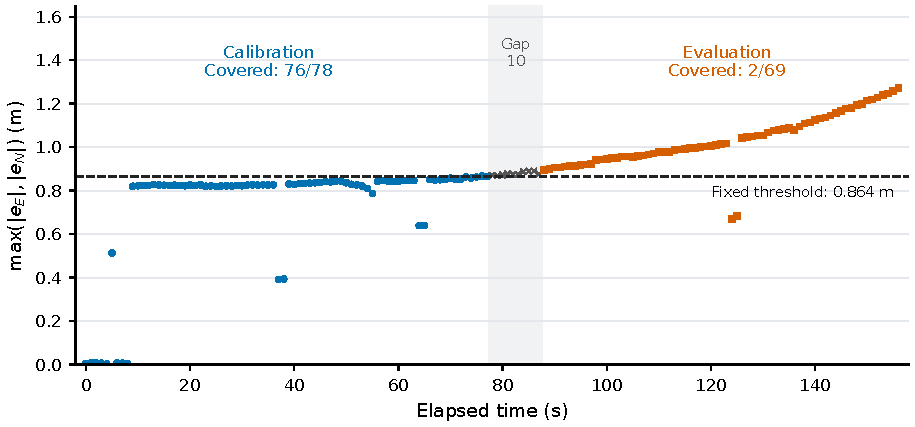
\includegraphics[width=\linewidth]{../figures/receiver_diagnostic.pdf}
\caption{Horizontal residual diagnostic for one stationary receiver. All 157 matched epochs are plotted, with a dashed line showing the 0.863506 m square half-width obtained from the calibration segment. Serial dependence and combined processing prevent interpreting this as online coverage performance.}\label{fig:receiver}
\end{figure}
